\let\negthickspace\undefined
\documentclass[journal,12pt,twocolumn]{IEEEtran}
\usepackage{cite}
\usepackage{amsmath,amssymb,amsfonts,amsthm}
\usepackage{algorithmic}
\usepackage{graphicx}
\usepackage{textcomp}
\usepackage{xcolor}
\usepackage{txfonts}
\usepackage{listings}
\usepackage{enumitem}
\usepackage{mathtools}
\usepackage{gensymb}
\usepackage{comment}
\usepackage[breaklinks=true]{hyperref}
\usepackage{tkz-euclide} 
\usepackage{listings}
\usepackage{gvv}                                        
\def\inputGnumericTable{}                                 
\usepackage[latin1]{inputenc}                                
\usepackage{color}                                            
\usepackage{array}                                            
\usepackage{longtable}                                       
\usepackage{calc}                                             
\usepackage{multirow}                                         
\usepackage{hhline}                                           
\usepackage{ifthen}                                           
\usepackage{lscape}
\usepackage{tfrupee}

\newtheorem{theorem}{Theorem}[section]
\newtheorem{problem}{Problem}
\newtheorem{proposition}{Proposition}[section]
\newtheorem{lemma}{Lemma}[section]
\newtheorem{corollary}[theorem]{Corollary}
\newtheorem{example}{Example}[section]
\newtheorem{definition}[problem]{Definition}
\newcommand{\BEQA}{\begin{eqnarray}}
\newcommand{\EEQA}{\end{eqnarray}}
\newcommand{\define}{\stackrel{\triangle}{=}}
\theoremstyle{remark}
\newtheorem{rem}{Remark}
\begin{document}

\bibliographystyle{IEEEtran}
\vspace{3cm}

\title{10.5.3.15}
\author{EE23BTECH11062 - V MANAS}
\maketitle
\newpage

\bigskip

\renewcommand{\thefigure}{\arabic{figure}}
\renewcommand{\thetable}{\arabic{table}}
\textbf{Question}:\\A contract on construction job specifies a penalty for delay of completion beyond a certain date as follows: \rupee $200$ for the first day, \rupee $250$ for the second day, \rupee $300$ for the third day, etc., the penalty for each succeeding day being \rupee $50$ more than for the preceding day.How much money the contractor has to pay as penalty, if he has delayed the work by $30$ days?\\
\textbf{Solution}:
\begin{table}[h]
    \centering
    \begin{tabular}{|c|c|c|c}
    \hline
    \textbf{Variable} & \textbf{Description} & \textbf{Values}\\
    \hline
    $G_o$ & overall transfer function & 1\\
    \hline
    $G_p$ & process transfer function & \\
    \hline
    $G_c$ & proportional controller transfer function & \\
    \hline
    $K_c$ & gain of the proportional controller & \\
    \hline
\end{tabular}

    \caption{Variables Used}
    \label{tab:table_10.5.3.15}
\end{table}
\begin{figure}[h]
    \centering
    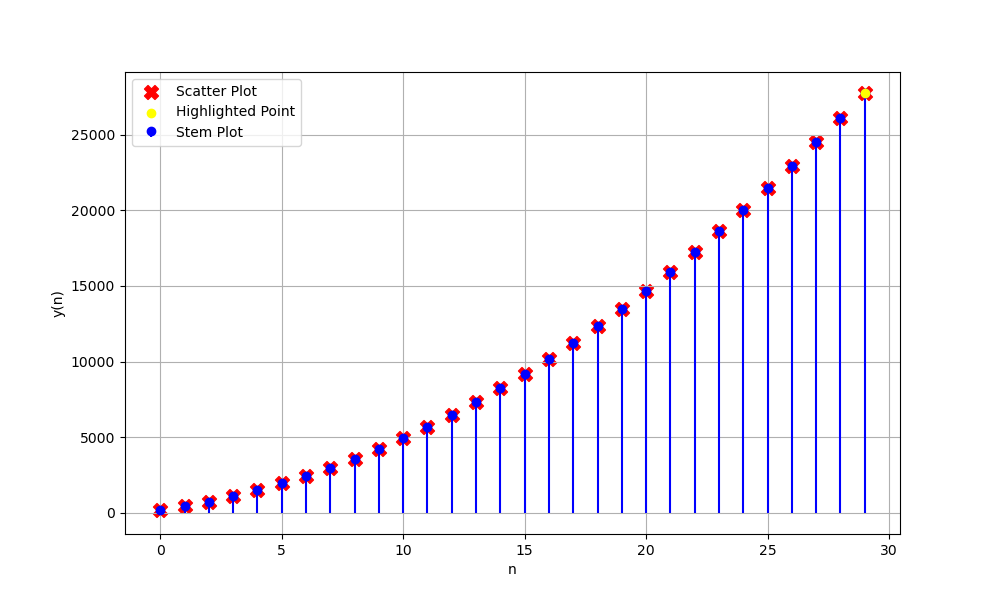
\includegraphics[width=1.1\linewidth]{figs/graph.png}
    \caption{Stem Plot of y(n)}
    \label{stemplot1}
\end{figure}\\
From equation(\ref{eq:apz})
\begin{align}
\implies X(z)&=\frac{200}{1-z^{-1}}+\frac{200z^{-1}}{(1-z^{-1})^2}\:\:
\quad\abs{z}>\abs{1}
\end{align}
\begin{align}
y\brak{n}&=x\brak{n}*u\brak{n}\\
Y\brak{z}&=X\brak{z}\,U\brak{z}\\
\implies Y\brak{z}&=\brak{\frac{200}{1-z^{-1}}+\frac{50z^{-1}}{\brak{1-
z^{-1}}^2}}\brak{\frac{1}{1-z^{-1}}}\\
&=\frac{200}{\brak{1-z^{-1}}^2}+\frac{50z^{-1}}{\brak{1-z^{-1}}^3}
\end{align}
Contour integration to find z transform
\begin{align}
y(29)&=\frac{1}{2{\pi}j}{\oint_c}Y\brak{Z}z^{28}dz\\
&=\frac{1}{2{\pi}j}{\oint_c}{\frac{(200-150z^{-1})z^{28}}{\brak{1-z^{-1}}^{3}}}
\end{align}
pole at 1 repeated 3 times
\begin{align}
\therefore m&=3\\
R&=\frac{1}{\brak{m-1}!}\lim_{z\to a}\frac{d^{m-1}}{dz^{m-1}}\brak{\brak{z
a}^mf{\brak{z}}}\\
&=\frac{1}{\brak{2!}}\lim_{z\to 1}\frac{d^2}{dz^2}\brak{\brak{z-1}^{3}\frac{(200-150z^{-1})z^{28}}{\brak{1-z^{-1}}^3}}\\
&=\lim_{z\to1}\frac{d^2}{dz^2}\brak{100-75z^{-1}}z^{31}
\end{align}
\begin{align}
\implies y(n)&=27750
\end{align}


\end{document}
